
% THIS IS SIGPROC-SP.TEX - VERSION 3.1
% WORKS WITH V3.2SP OF ACM_PROC_ARTICLE-SP.CLS
% APRIL 2009
%
% It is an example file showing how to use the 'acm_proc_article-sp.cls' V3.2SP
% LaTeX2e document class file for Conference Proceedings submissions.
% ----------------------------------------------------------------------------------------------------------------
% This .tex file (and associated .cls V3.2SP) *DOES NOT* produce:
%       1) The Permission Statement
%       2) The Conference (location) Info information
%       3) The Copyright Line with ACM data
%       4) Page numbering
% ---------------------------------------------------------------------------------------------------------------
% It is an example which *does* use the .bib file (from which the .bbl file
% is produced).
% REMEMBER HOWEVER: After having produced the .bbl file,
% and prior to final submission,
% you need to 'insert'  your .bbl file into your source .tex file so as to provide
% ONE 'self-contained' source file.
%
% Questions regarding SIGS should be sent to
% Adrienne Griscti ---> griscti@acm.org
%
% Questions/suggestions regarding the guidelines, .tex and .cls files, etc. to
% Gerald Murray ---> murray@hq.acm.org
%
% For tracking purposes - this is V3.1SP - APRIL 2009

\documentclass{acm_proc_article-sp}

\usepackage{multirow}
\usepackage{subfigure}
\usepackage{graphicx}
\usepackage{graphics}
\usepackage{rotating}
\usepackage{verbatim}
\usepackage{float}
\usepackage{url}
\usepackage{tabularx}
\usepackage{amsmath}
\usepackage{listings}
\usepackage{color}
\definecolor{javared}{rgb}{0.6,0,0} % for strings
\definecolor{javagreen}{rgb}{0.25,0.5,0.35} % comments
\definecolor{javapurple}{rgb}{0.5,0,0.35} % keywords
\definecolor{javadocblue}{rgb}{0.25,0.35,0.75} % javadoc
 
\lstset{language=Java,
basicstyle=\ttfamily,
keywordstyle=\color{javapurple}\bfseries,
stringstyle=\color{javared},
commentstyle=\color{javagreen},
morecomment=[s][\color{javadocblue}]{/**}{*/},
%numbers=left,
numberstyle=\tiny\color{black},
stepnumber=2,
numbersep=10pt,
tabsize=4,
showspaces=false,
showstringspaces=false}



\restylefloat{table}

\hyphenation{op-tical net-works semi-conduc-tor}



\begin{document}



\title{Dirt Spot Sweeping Random Strategy}


\numberofauthors{2} %  in this sample file, there are a *total*
% of EIGHT authors. SIX appear on the 'first-page' (for formatting
% reasons) and the remaining two appear in the \additionalauthors section.
%
\author{
% You can go ahead and credit any number of authors here,
% e.g. one 'row of three' or two rows (consisting of one row of three
% and a second row of one, two or three).
%
% The command \alignauthor (no curly braces needed) should
% precede each author name, affiliation/snail-mail address and
% e-mail address. Additionally, tag each line of
% affiliation/address with \affaddr, and tag the
% e-mail address with \email.
%
% 1st. author
\alignauthor
Mian Asbat Ahmad\\
       \affaddr{Department of Computer Science}\\
       \affaddr{The University of York}\\
       \affaddr{York, United Kingdom}\\
       \email{mian.ahmad@york.ac.uk}
% Please Dr. Manuel, add your abb details. I am not able to create table here because of the format. Thanks.
\alignauthor
Manuel Oriol \\
       \affaddr{Department of Computer Science}\\
       \affaddr{The University of York}\\
       \affaddr{York, United Kingdom}\\
       \email{manuel.oriol@york.ac.uk}
}



\maketitle
\begin{abstract}
This paper presents an enhanced and improved form of automated random testing, called the Dirt Spot Sweeping Random (DSSR) strategy. DSSR is a new strategy that takes the assumption that a number of failure domains are contiguous.
DSSR starts as a regular random+ testing session --- a random testing session with some preference for boundary values. 
When a failure is found, it increases the chances of using neighbouring values in subsequent tests, thus slowly sweeping around the failure found in hope of finding failures from a different kind in its vicinity.

DSSR was implemented within the YETI random testing tool. We evaluate DSSR against random+ and pure random strategies by testing 60 classes with one million ($10^5$) calls for each session 30 times for each strategy.
We found that for 72\% of the classes all three strategies find the same unique failures, for remaining 28\% DSSR perform better (up to as much as 33\%) then random strategy and (up to as much as 17\%) then random+ strategy.
Overall, DSSR also found 27 more unique failures than random and 11 more unique failures than random+ strategy.
\end{abstract}

%A category including the fourth, optional field follows...
\category{D.2.5}{Software Engineering}{Metrics}[complexity measures, performance measures]

\terms{Comparison, Verification, }

\keywords{software testing, automated random testing, comparative analysis} % NOT required for Proceedings


%%%%%%%%%%%%%%%%%    INTRODUCTION   %%%%%%%%%%%%%%%%%%%%
\section{Introduction}\label{sec:intro}
Success of a software testing technique is mainly based on the number of faults it discovers in the Software Under Test (SUT). An efficient testing process discovers the maximum number of faults in a minimum possible amount of time. Exhaustive testing, where software is tested against all possible inputs, is in most cases not feasible because of the size of the input domain, limited resources and strict time constraints. Therefore, strategies in automated software testing tools are developed with the aim to select more fault-finding test input from the input domain for a given SUT. Producing such targeted test input is difficult because each system has its own requirements and functionality.

Chan et al.~\cite{Chan1996} discovered that there are patterns of failure-causing inputs across the input domain. They divided the patterns into point, block and strip patterns on the basis of their occurrence across the input domain. Chen et al.~\cite{Chen2008} found that the performance of random testing can be increased by slightly altering the technique of test case selection. In adaptive random testing, they found that the performance of random testing increases by up to 50\% when test input is selected evenly across the whole input domain. This was mainly attributed to the better distribution of input which increased the chance of selecting inputs from failure patterns. Similarly Restricted Random Testing \cite{Chan2002}, Feedback directed Random Test Generation \cite{Pacheco2007a}, Mirror Adaptive Random Testing \cite{Chen2003} and Quasi Random Testing \cite{Chen2005} also stress the need for test case selection covering the whole input domain to improve results.

In this paper we take the assumption that for a significant number of classes failure domains are contiguous or are very close by. From this assumption, we devised the Dirt Spot Sweeping\footnote{The name refers to the cleaning robots strategy which insists on places where dirt has been found in large amount.} Random strategy (DSSR) which starts as a random+ strategy --- a random strategy focusing more on boundary values. When it finds a new failure, it then increases the chances of finding more faults using neighbouring values. Note that, similarly to previous studies~\cite{Oriol2012} we approximate faults with unique failures. Of course, since this strategy is also a random testing strategy, it has the potential to find all unique failures in the program, but we expect it to be faster at finding unique failures for classes in which failure domains are contiguous than the pure random (R) and random+ (R+) strategies.

We implemented DSSR as a strategy for the random testing tool YETI\footnote{\url{http://www.yetitest.org}}. To evaluate our approach, we tested thirty times each one of 60 classes of 32 different projects from the Qualitas Corpus\footnote{\url{http://www.qualitascorpus.com}} with each of the three strategies DSSR, R, and R+. We found that for 72\% of the classes all three strategies find the same unique failures, for remaining 28\% DSSR perform better (up to as much as 33\%) then random strategy and (up to as much as 17\%) then random+ strategy.
Overall, DSSR also found 27 more unique failures than random and 11 more unique failures than random+.


The rest of this paper is organised as follows:
Section~\ref{sec:dssr} describes the DSSR strategy. Section~\ref{sec:imp} presents our implementation of the strategy. Section~\ref{sec:eval} explains our experimental setup. Section~\ref{sec:res} shows the results of our experiments. Section~\ref{sec:discussion} discusses the results. Section~\ref{sec:rw} presents related work and we conclude in Section~\ref{sec:conc}.




%%%%%%%%%%%%%%%%%    DIRT SPOT SWEEPING STRATEGY  %%%%%%%%%%%%%%%

\section{Dirt Spot Sweeping Random \\ Strategy}\label{sec:dssr}
The Dirt Spot Sweeping Random strategy (DSSR) is a new strategy which combines the random+ strategy with a dirt spot sweeping functionality. The strategy is based on two intuitions. First, boundaries have interesting values and using these values in isolation can provide high impact on test results. Second, faults and unique failures reside in contiguous blocks and stripes. If this is the case, DSSR increases the performance of the test strategy. Each strategy is briefly explained as follows.

\subsection{Random Strategy (R)}
The pure random strategy is a black-box testing technique in which the SUT is executed using randomly selected test data. Test results obtained are compared to the defined oracle, using SUT specifications in the form of contracts or assertions. In the absence of contracts and assertions the exceptions defined by the programming language are used as test oracles. 

Because of its black-box testing nature, this strategy is particularly effective in testing softwares where the developers want to keep the source code secret~\cite{Chen2010}. The generation of random test data is comparatively cheap and does not require too much intellectual and computation efforts~\cite{Ciupa2009, Ciupa2008}. It is mainly for this reason that various researchers have recommended this strategy for automatic testing tools \cite{Ciupa2008a}. YETI \cite{Oriol2010a, Oriol2010}, AutoTest \cite{Leitner2007, Ciupa2007}, QuickCheck \cite{Claessen2000}, Randoop \cite{Pacheco2007}, Jartage \cite{Oriat2004} are some of the most common automated testing tools based on random strategy.

\indent Efficiency of random testing was made suspicious with the intuitive statement of Myers \cite{Myers2004} who termed random testing as one of the poorest methods for software testing. However, experiments performed by various researchers, \cite{Ciupa2007, Duran1981, Duran1984, Hamlet1994, Ntafos2001} have experimentally proven that random testing is simple to implement, cost effective, highly efficient and free from human bias as compared to its rival techniques.

Because programs tested at random typically fail a large number of times (there are a large number of calls), it is necessary to cluster failures that likely represent the same fault. The traditional way of doing it is to compare the full stack traces and error types and use this as an equivalence class~\cite{Ciupa2007,Oriol2012} called a unique failure. This way of grouping failures is also used for random+ and DSSR.

\subsection{Random Plus Strategy (R+)}
The random+ strategy~\cite{Leitner2007} is an extension of the pure random strategy. It uses some special pre-defined values which can be simple boundary values or values that have high tendency of finding faults in the SUT. Boundary values~\cite{Beizer1990} are the values on the start and end of a particular type. For instance, such values for \verb+int+ could be \verb+MAX_INT+, \verb+MAX_INT-1+, \verb+MIN_INT+, \verb-MIN_INT+1-, \verb+-1+, \verb+0+, \verb+1+ etc.



Similarly, the tester might also add some other special values that he considers effective in finding faults for the current SUT. For example, if a program under test has a loop from -50 to 50 then the tester can add -55 to -45, -5 to 5 and 45 to 55 to the pre-defined list of special values in order to be selected for a test. This static list of interesting values is manually updated before the start of the test and has slightly high priority than selection of random values because of more relevance and high chances of finding faults for the given SUT. These special values have high impact on the results particularly detecting problems in specifications~\cite{Ciupa2008}.


\subsection{Dirt Spot Sweeping}
Chan et al.~\cite{Chan1996} found that there are patterns of failure-causing inputs across the input domain. Figure \ref{fig:patterns} shows these patterns for two dimensional input domain. They divided these patterns into three types called points, block and strip patterns. The black area (Points, block and strip) inside the box show the input which causes the system to fail while white area inside the box represent the genuine input. Boundary of the box (black solid line) surrounds the complete input domain and also represents the boundary values. They also argue that a strategy has more chances of hitting these fault patterns if test cases far away from each other are selected. Other researchers~\cite{Chan2002, Chen2003, Chen2005}, also tried to generate test cases further away from one another targeting these patterns and achieved higher performance. High performance of these strategies indicate that faults more often occur contiguous across the input domain. In Dirt Spot Sweeping we propose that if test case reveal a fault then for the next test case it may not look farthest away from itself because it is in the fault region instead it may pick the closest test case to find another fault from the same region.

\begin{figure}[ht]                                    
\centering
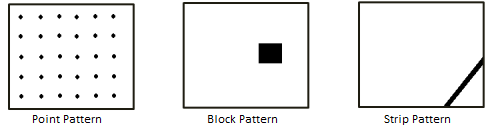
\includegraphics[width= 8cm,height=2.5cm]{ART_Patterns.png}
\caption{Failure patterns across input domain~\cite{Chen2008}}
\label{fig:patterns}
\end{figure}

Dirt spot sweeping is the part of DSSR strategy that comes into action when a failure is found in the system. On finding a failure, it immediately adds the value causing the failure and its neighbouring values to the already existing list of interesting values. For example in a program if the \verb+int+ type value 50 causes a failure in the system then spot sweeping will add values from 47 to 53 to the list of interesting values. If the failure lies in the block or strip pattern, then adding its neighbours will explore other failures present in that block or strip. As against random plus where the list of interesting values remain static, the list of interesting values is dynamic and changes during the test execution of each program in the DSSR strategy.

\begin{figure}[ht]
\centering
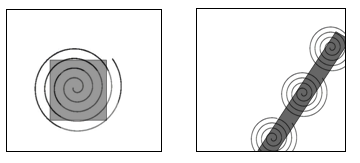
\includegraphics[width=8cm,height=2.2cm]{block2.png}
\caption{DSSR covering block and strip pattern}
\label{fig:block2}
\end{figure}

Figure \ref{fig:block2} shows how dirt spot sweeping explores the failures residing in the block and strip patterns of a program. The failure coverage from the pattern is shown in spiral form because first failure will lead to second, second to third and so on till the end. In case the failure is positioned on the point pattern then the added values will not be very effective because point pattern is only an arbitrary failure point in the whole input domain.

\subsection{Structure of the Dirt Spot Sweeping \\ Random Strategy}

In this process, the strategy continuously tracks the number of failures during the execution of the test session. To keep the system fast this tracking is done in a very effective way with zero or minimum overhead~\cite{Leitner2009}. The execution of test is performed normally until a failure is found in the SUT. Then the program does not only copy the values that lead to the failure, but also copies its surrounding values to the variable list of interesting values. 

\begin{figure}[ht]
\centering
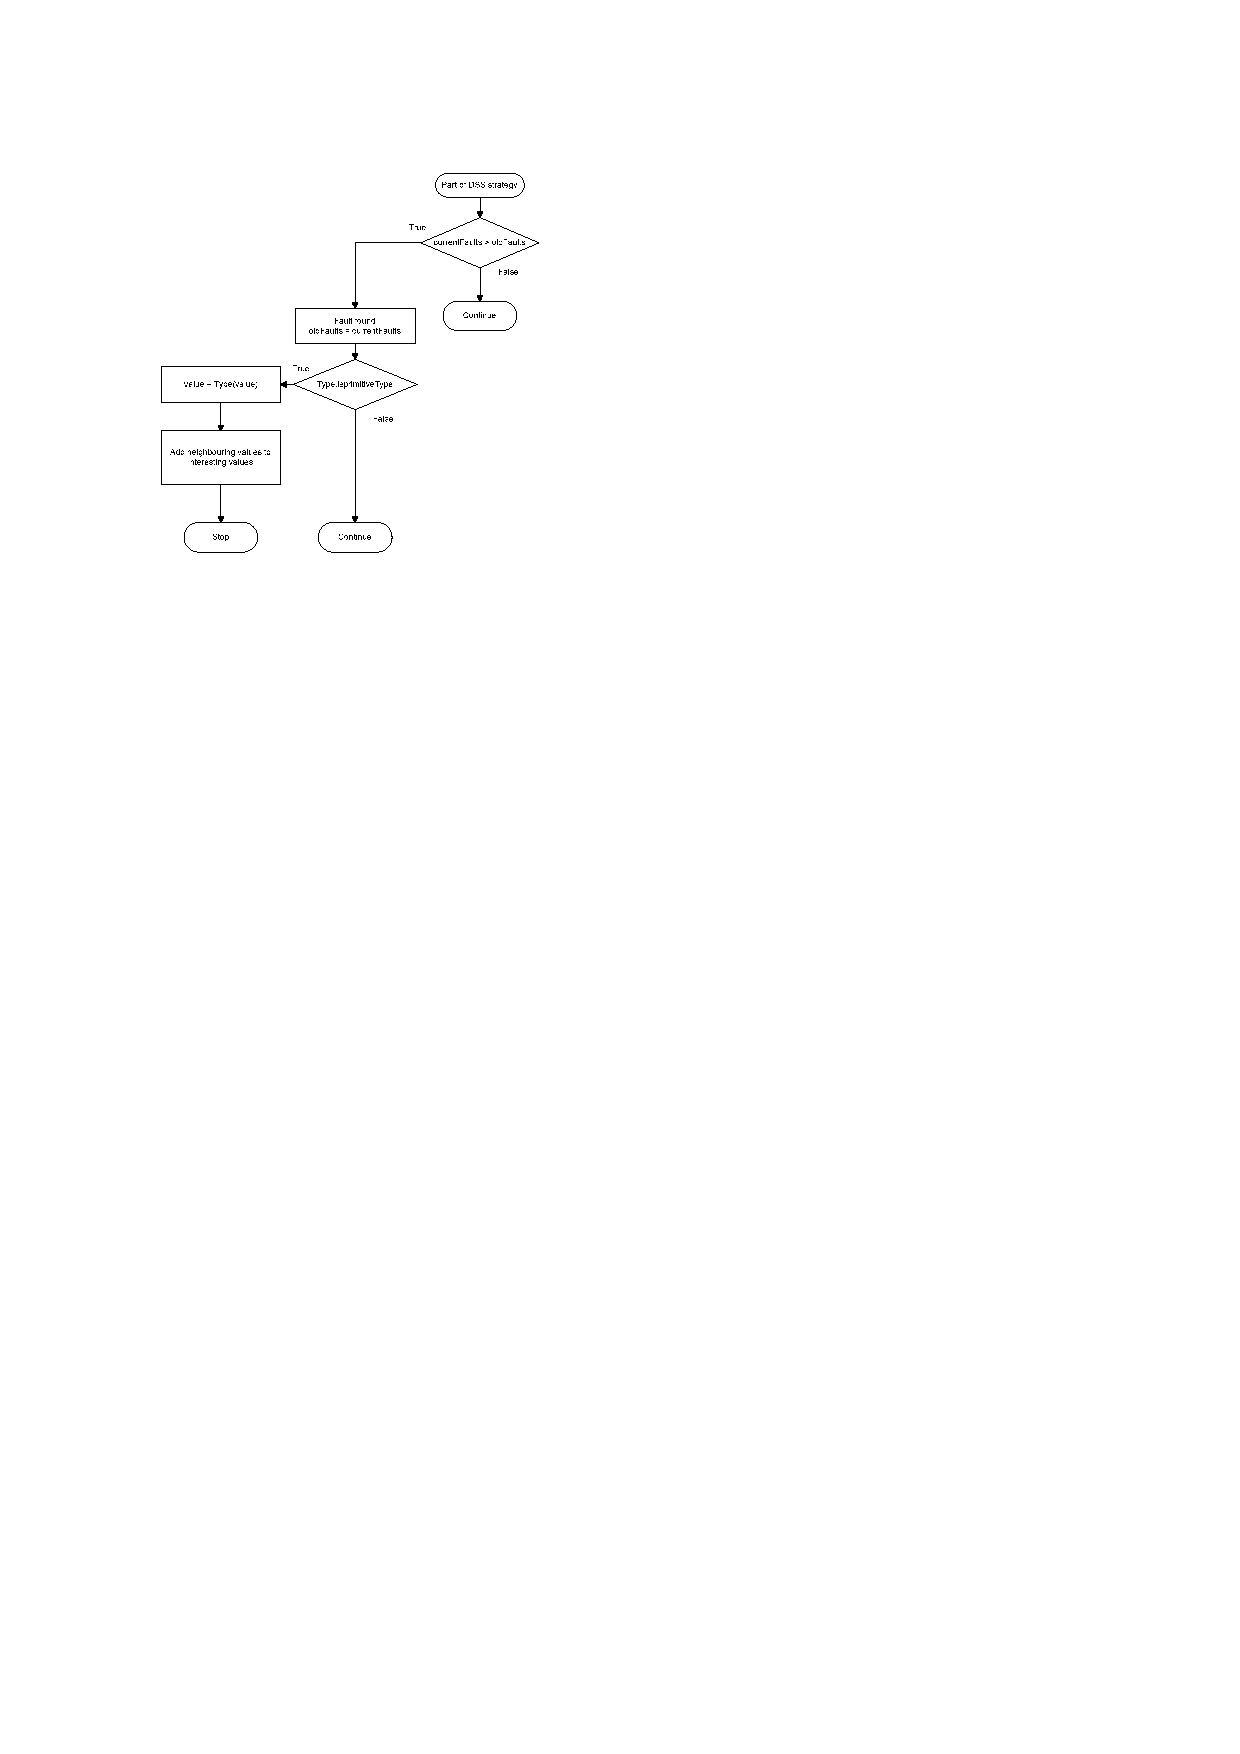
\includegraphics[width=\columnwidth]{flowchart1.pdf}
\caption{Working mechanism of DSSR Strategy}
\label{fig:Working_DSSS}
\end{figure}

As presented in the flowchart in Figure~\ref{fig:Working_DSSS}, if the failure finding value is of primitive type then the DSSR finds the type of the value and add values only of that particular type to the interesting values. Addition of these values increases the size of the list of interesting values that provide relevant test data for the remaining test session and the new generated test cases are more targeted towards finding new failures in the given SUT around pre-existing failures.

Boundary values and other special values that have a high tendency of finding faults in the SUT are added to the list by random plus strategy prior to the start of test session where as to sweep the failure pattern, the fault-finding value and its surrounding values are added at runtime after a failure is found. Table \ref{table:addvalues} presents the values that are added to the list of interesting values when a failure is found. In the table the test value is represented by X where X can be int, double, float, long, byte, short, char and String. All values are converted to their respective types before adding to the list of interesting values and vice versa.

\begin{table}[ht]
%\scriptsize
\caption{Neighbouring values for primitive types and String} % title of Table
\centering % used for centering table
\begin{tabular}{| l | l |} % centered columns (4 columns)
\hline\hline %inserts double horizontal lines
Type & Values to be added\\ [0.5ex] % inserts table
%heading
\hline % inserts single horizontal line
\multirow{1}{*}{X is int, double, float, } & ~ X,  X+1, X+2, X-1, X-2 \\ % inserting body of the
\multirow{1}{*}{long, byte, short \& char} &  \\ 

\hline
\multirow{8}{*}{X is String} & ~ X\\ % inserting body of the table

& ~ X + ``  "\\ % inserting body of the table
& ~ ``  " + X \\ % inserting body of the table
& ~ X.toUpperCase() \\
& ~ X.toLowerCase() \\
& ~ X.trim() \\
& ~ X.substring(2) \\
& ~ X.substring(1, X.length()-1) \\[1ex]
\hline
\hline %inserts single line
\end{tabular}
\bigskip
\label{table:addvalues} % is used to refer this table in the text
\end{table}





%%%%%%%%%%%%%%%%%%%%%%%%%%%%% EXPLANATION OF DSSR STRATEGY %%%%%%%%%%%%%%%%%%%%%%%%%%


\subsection{Explanation of DSSR on a concrete \\ example}
The DSSR strategy is explained through a simple program seeded with at least three faults. The first fault is a division by zero exception denoted 1 while the second and third are failing assertion statements denoted 2 and 3 in the following program.  Below we describe how the DSSR strategy perform execution when the following class is expose to testing.

\begin{lstlisting}
/** 
* Calculate square of given number 
* and verify results. 
* The code contain 3 faults.
* @author (Mian and Manuel)
*/
public class Math1 {
 public void calc (int num1) {
  // Square num1 and store result. 
  int result1 = num1 * num1;
  int result2 = result1 / num1; // 1
  assert Math.sqrt(result1) == num1; // 2
  assert result1 >= num1; // 3
 } 
}
\end{lstlisting}

In the above code, one primitive variable of type \verb+int+ is used, therefore, the input domain for DSSR strategy is from \verb+-2,147,483,648 to 2,147,483,647+. The strategy further selects some values (\verb+0, Integer.MIN_VALUE+ and\\ \verb+Integer.MAX_VALUE+) as interesting values which are prioritised for selection as inputs. 
As the test starts, three faults are quickly discovered by DSSR strategy in the following order.

\indent \textbf{Fault 1:} The DSSR strategy might select value \verb+0+ for variable \verb+num1+  in the first test case because \verb+0+ is available in the list of interesting values and therefore its priority is higher than other values. This will cause Java to generate division by zero exception.

\indent \textbf{Fault 2:} After catching the first fault, the strategy adds it and its surrounding values to the list of interesting values which includes \verb+0, 1, 2, 3 and -1, -2, -3+ in this case. In the second test case DSSR strategy may pick \verb+-3+ as a test value and lead to the second fault where assertion (2) fails because the square root of \verb+9+ will be \verb+3+ instead of the input value -3.

\indent \textbf{Fault 3:} After few tests DSSR strategy may select \\ \verb+Integer.MAX_VALUE+ for variable \verb+num1+  from the list of interesting values which will lead to the 3rd fault because \verb+result1+ will not be able to store the square of \\ \verb+Integer.MAX_VALUE+. Instead of the actual square value Java assigns a negative value (Java language rule) to variable result1 that will lead to the violation of the next assertion (3).

The process above explains that the pre-defined values including border values, fault-finding values and the surrounding values lead to the available faults quickly and in small number of tests as compared to random and random+ strategy. Random and random+ takes longer to discover the second and third fault because they start again searching for new unique failures randomly although the remaining faults are very close to the first one. 


%%%%%%%%%%%%%%%%%    IMPLEMENTATION OF DSSR STRATEGY   %%%%%%%%%%%%


\section{Implementation of the DSSR \\ strategy}\label{sec:imp}

As mentioned previously, the implementation of the DSSR strategy is made in the YETI open-source automated random testing tool. YETI is developed in Java and capable of testing systems developed in procedural, functional and object-oriented languages. Its language-agnostic meta model enables it to test programs written in multiple languages including Java, C\#, JML and .Net. The core features of YETI include easy extensibility for future growth, speed of up to one million calls per minute on java code, real time logging, real time GUI support, ability to test programs using multiple strategies, and auto generation of test report at the end of the testing sessions. For large-scale testing there is a cloud-enabled version of YETI that is capable of executing parallel test sessions in Cloud~\cite{Oriol2010}. A number of hitherto faults have successfully been found by YETI in various production softwares~\cite{Oriol2012, Oriol2011}.

YETI can be divided into three decoupled main parts: the core infrastructure, language-specific bindings and strategies. The core infrastructure contains representation for routines, a group of types and a pool of specific type objects. The language specific bindings contain the code to make the call and process the results. The strategies section defines the procedure of how to select the modules (classes) from the project, how to select routines (methods) from these modules and how to generate values for the instances involved inside these routines. The most common strategies are random and random+. 

By default, YETI uses the random+ strategy if no particular strategy is defined during test initialisation. It also enables the user to control the probability of using null values and the percentage of newly created objects for each test session. YETI provides an interactive Graphical User Interface (GUI) in which users can see the progress of the current test in real time. In addition to the GUI, YETI also provides extensive logs of the test session for more in-depth analysis.

The DSSR strategy has then been added as an extension of YetiRandomStrategy, which in itself is an extension of an abstract class YetiStrategy. The class hierarchy is shown in Figure \ref{fig:hierarchyofDSSR}.

\begin{figure}[h]
\centering
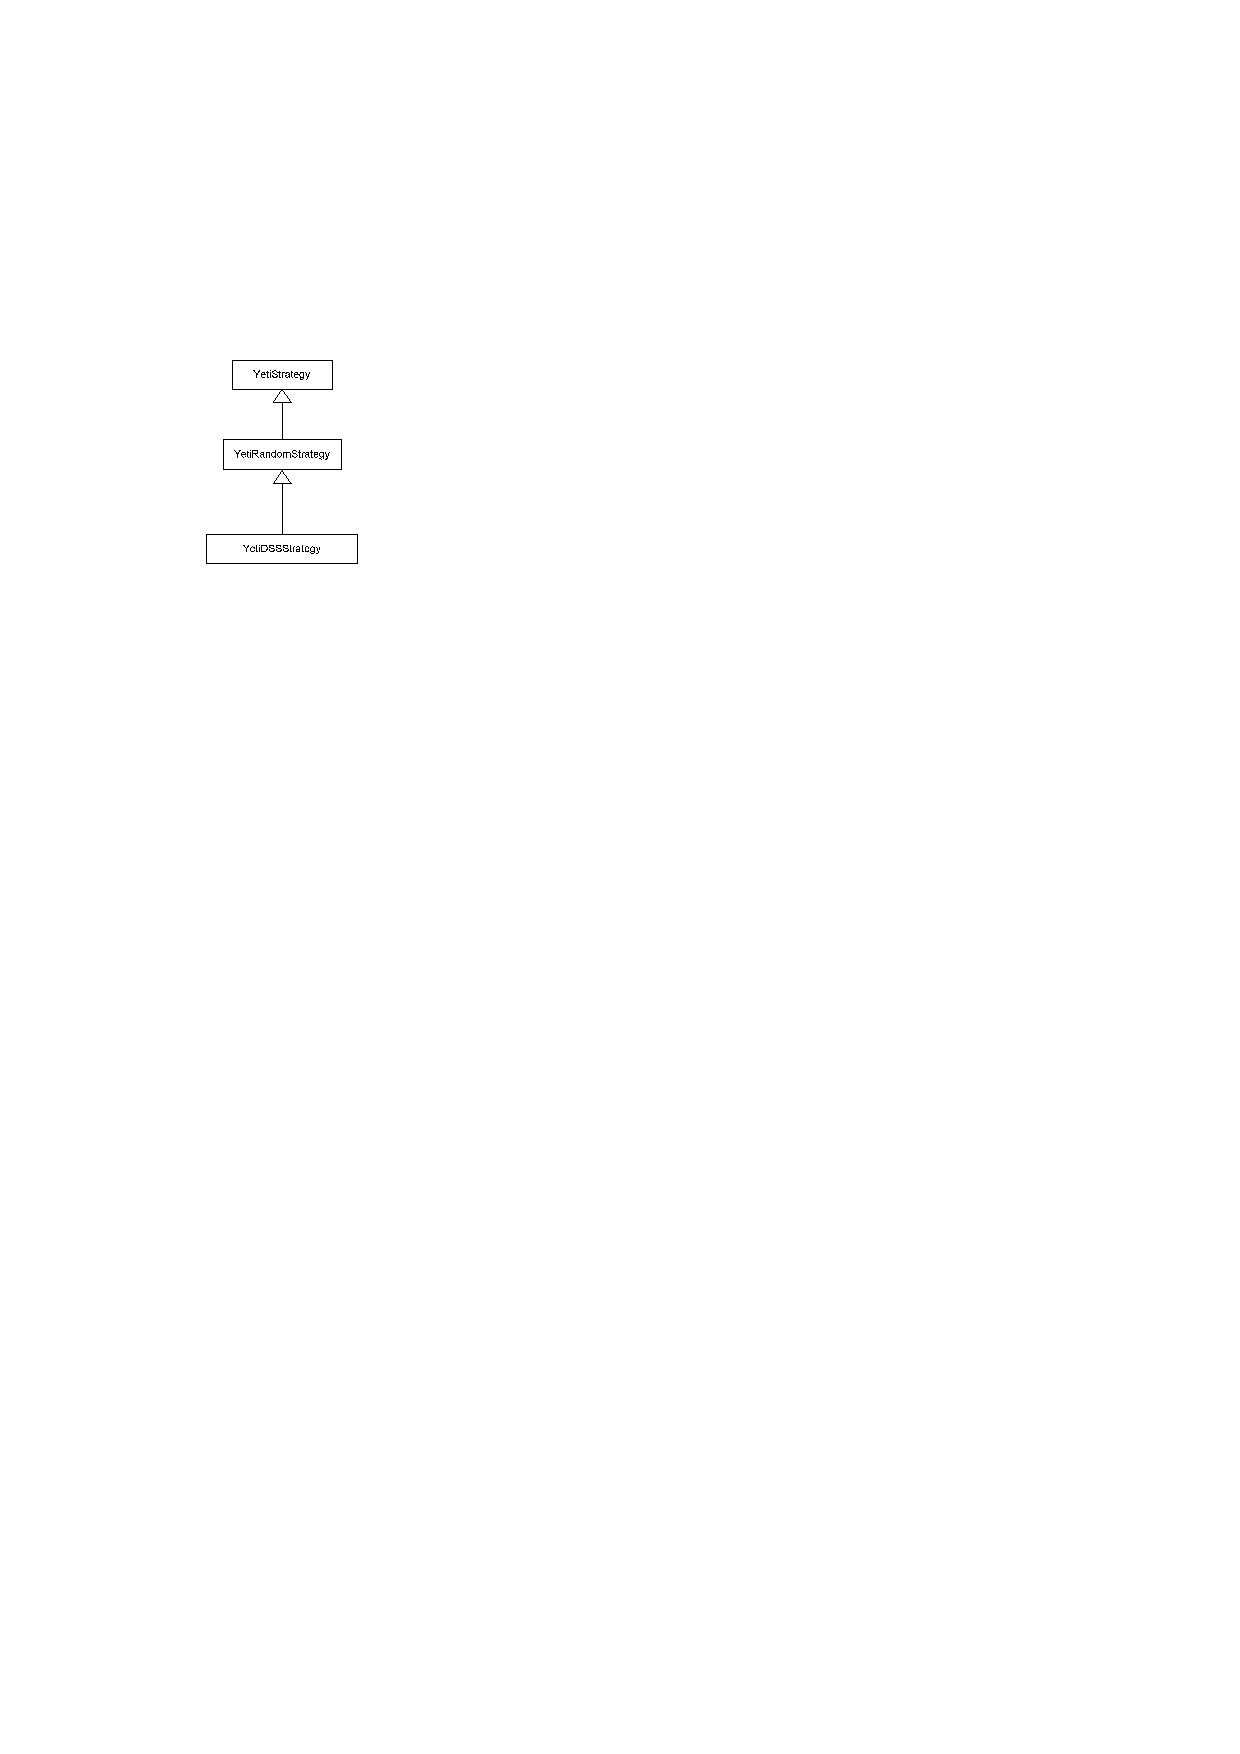
\includegraphics[width=4cm,height=5cm]{hierarchy.pdf}
\caption{Class Hierarchy of DSSR in YETI}
\label{fig:hierarchyofDSSR}
\end{figure}





%%%%%%%%%%%%%%%%%    EVALUATION   %%%%%%%%%%%%%%%%%%%%


\section{Evaluation}\label{sec:eval}

To evaluate the DSSR strategy, we compare its performance to the performance of both pure random testing (R) and the random+ (R+)~\cite{Leitner2007} strategy. General factors such as system software and hardware as well as the YETI specific factors like percentage of null values, percentage of newly created objects and interesting value injection probability have the same values for the experiments.

\subsection{Research questions}
To evaluate the DSSR strategy and its usefulness, we set out to answer the following research questions:
\begin{enumerate}
\item Is any of the three strategies R, R+ and DSSR provide better results than the other two?
\item Is there a subset of the classes for which R, R+, or DSSR provide better results than the other two?
\item If such categories exist, what are their sizes and how do they compare and can we pick a default strategy according to this criterion?
\end{enumerate}



\subsection{Experiments}

To evaluate the performance of DSSR we performed extensive testing of programs from the Qualitas Corpus~\cite{Tempero2010a}. The Qualitas Corpus is a curated collection of open source java projects built with the aim of helping empirical research on  software engineering. These projects are collected in an organised form containing both the source and binary forms. The present evaluation uses version 20101126 which contains 106 open source java projects. For the experiments, 60 random classes from 32 random projects are selected. Name, version and size of the projects to which the classes belong are given in table~\ref{table:projects} while dentail for the classes is given in table~\ref{table:Results}. All the selected classes produced at least one fault and did not timeout with a testing session of maximum 10 minutes. Each class is tested thirty times with each strategy. Total number of Line of Code (LOC) tested in the experiments is 40,213. Per class LOC is given in column 3 of table~\ref{table:Results}. 

Each class is evaluated through $10^5$ calls in each testing session.\footnote{The total number of tests is thus $60\times 30\times 3 \times 10^5 = 540\times 10^6~tests$.} 
Because of the absence of the contracts and assertions in the code under test, similarly to previous approaches~\cite{Oriol2012}, we use undeclared exceptions to compute unique failures found.


\begin{table}[h]
\caption{Name and versions of 32 Projects randomly selected from the Qualitas Corpus for the experiments}
\centering
\begin{tabular}{rlrr}
S. No& 	Project Name	& 	Version		&	Size (MB)\\
1	&	apache-ant	&	1.8.1			&	59\\
2	&	antlr			&	3.2			&	13\\
3	&	aoi			&	2.8.1			&	35\\
4	&	argouml		&	0.30.2		&	112\\
5	&	artofillusion	&	281			&	5.4\\
6	&	aspectj		&	1.6.9			&	109.6\\
7	&	axion		&	1.0-M2		&	13.3\\
8	&	azureus		&	1			&	99.3\\
9	&	castor		&	1.3.1			&	63.2\\
10	&	cayenne		&	3.0.1			&	4.1\\
11	&	cobertura		&	1.9.4.1		&	26.5\\
12	&	colt			&	1.2.0			&	40\\
13	&	emma		&	2.0.5312		&	7.4\\
14	&	freecs		&	1.3.20100406	&	11.4\\
15	&	hibernate		&	3.6.0			&	733\\
16	&	hsqldb		&	2.0.0			&	53.9\\
17	&	itext			&	5.0.3			&	16.2\\
18	&	jasml		&	0.10			&	7.5 \\
19	&	jmoney		&	0.4.4			&	5.3\\
20	&	jruby			&	1.5.2			&	140.7\\
21	&	jsXe			&	04\_beta		&	19.9\\
22	&	quartz		&	1.8.3			&	20.4\\
23	&	sandmark		&	3.4			&	18.8\\
24	&	squirrel-sql	&	3.1.2			&	61.5\\
25	&	tapestry		&	5.1.0.5		&	69.2\\
26	&	tomcat		&	7.0.2			&	24.1\\
27	&	trove			&	2.1.0			&	18.2\\
28	&	velocity		&	1.6.4			&	27.1\\
29	&	weka		&	3.7.2			&	107\\
30	&	xalan		&	2.7.1			&	85.4\\
31	&	xerces		&	2.10.0		&	43.4\\
32	&	xmojo		&	5.0.0			&	15\\
\end{tabular}
\bigskip
\label{table:projects}
\end{table}



All tests are performed using a 64-bit Mac OS X Lion Version 10.7.4 running on 2 x 2.66 GHz 6-Core Intel Xeon with 6.00 GB (1333 MHz DDR3) of RAM. YETI runs on top of the Java\texttrademark  SE Runtime Environment [version 1.6.0\_35]. The machine took approximately 100 hours to process the experimental data.


\subsection{Performance measurement criteria}
Various measures including the E-measure, P-measure and F-measure have been used by researchers to find the effectiveness of the random test strategy. The E-measure (expected number of failures detected) and P-measure (probability of detecting at least one failure) were heavily criticised~\cite{Chen2008} and are not considered effective techniques for measuring efficiency of test strategy. The F-measure (number of test cases used to find the first fault) has been often used by researchers~\cite{Chen1996, Chen2004}. In our initial experiments the F-measure was used to evaluate the efficiency. Soon after a few experiments, it was realised that this was not the right choice because in some experiments the first strategy found the first fault quickly than the second strategy but on the completion of test session the first strategy found lower number of total faults than the second strategy. The preference to a strategy only because it found the first fault better without giving due consideration to the total number of faults was not fair~\cite{Liu2012}.


  
The literature review revealed that the F-measure is used where testing stops after identification of the first fault and the system is given back to the developers to remove the fault found. In such cases it make sense to use F-measure but nowadays automated testing tools test the whole system and print all of the faults found in one go therefore F-measure is not the favourable choice. Therefore in our experiments, performance of the strategy was measured by the maximum number of faults in a particular number of test calls \cite{Pacheco2007a, Ciupa2007, Ciupa2008b}. This measurement was found effective because it clearly measured the performance of the strategy when all the other factors were kept constant.

%%%%%%%%%%%%%%%%%    RESULTS   %%%%%%%%%%%%%%%%%%%%
\begin{figure*}[ht]
\centering
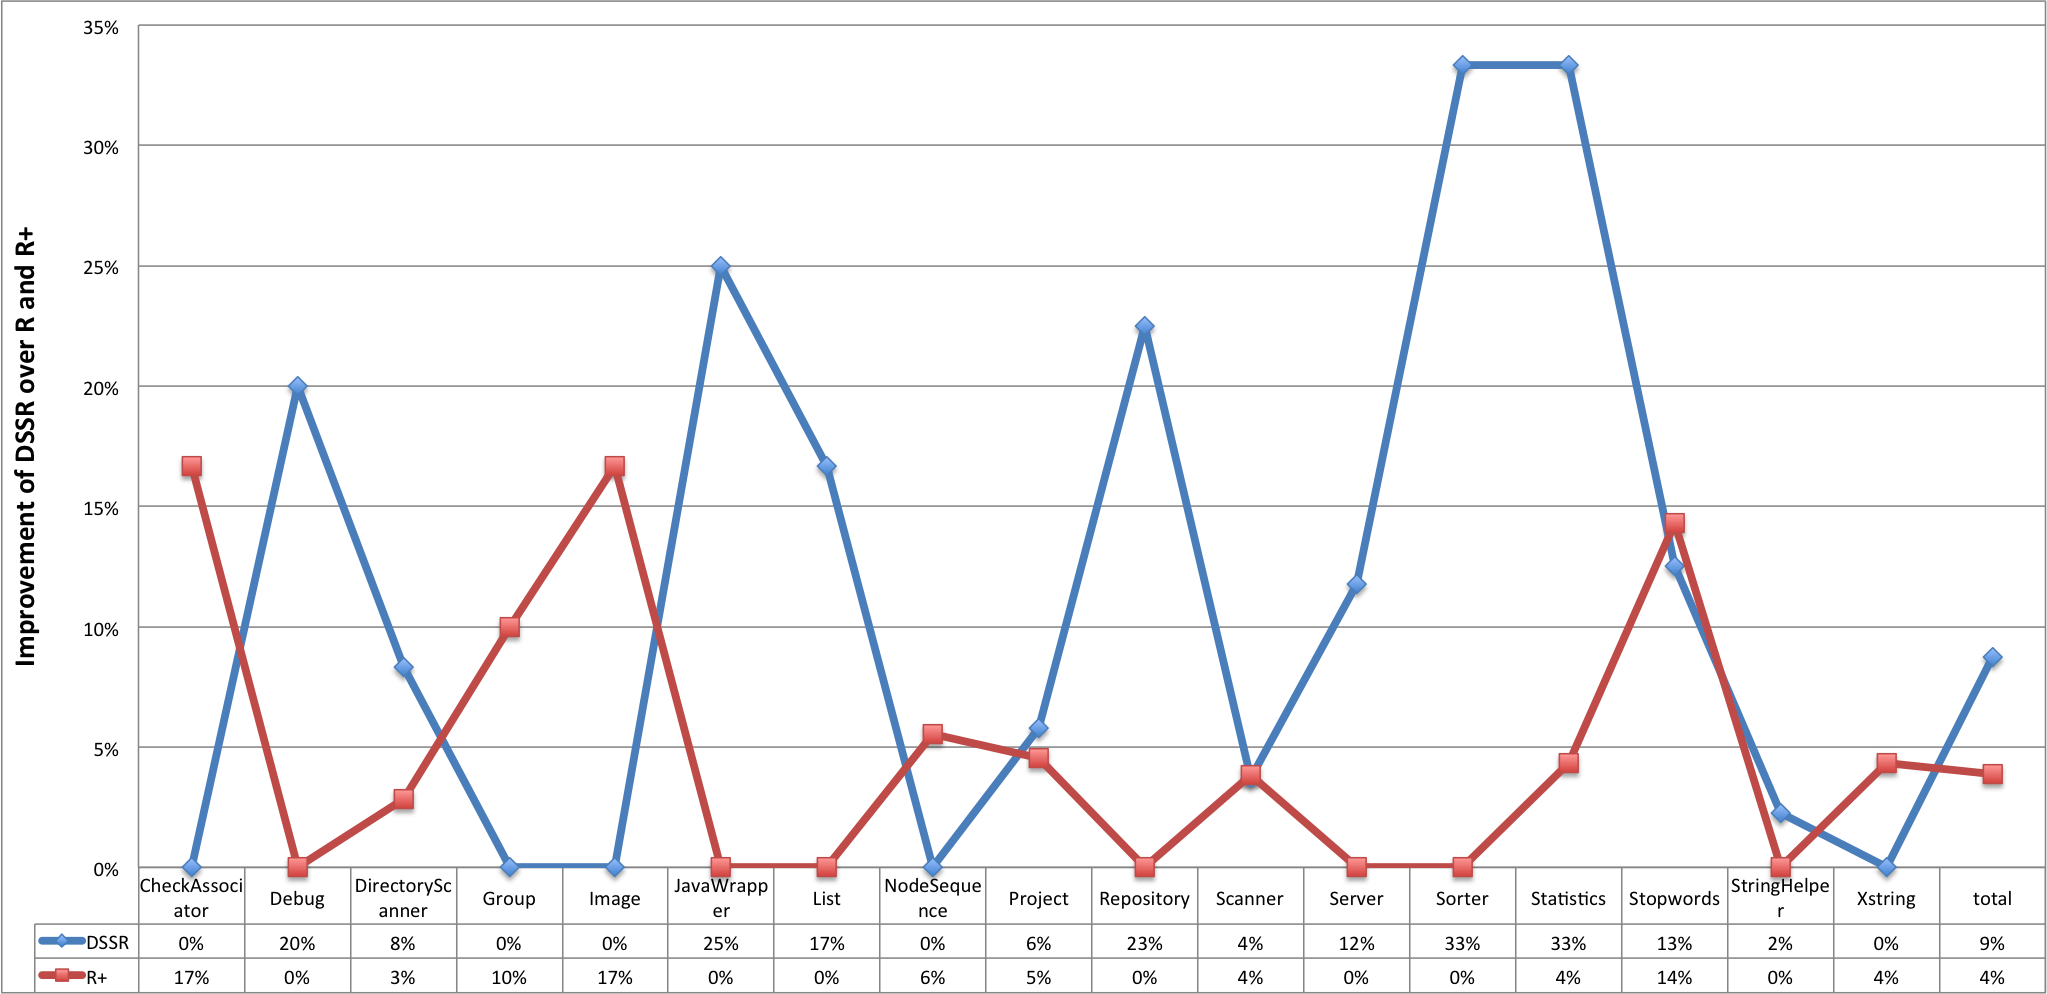
\includegraphics[width=18cm]{DssrImprove.png}
\caption{Improvement of DSSR strategy over Random and Random+ strategy.}
\label{fig:LineChart}
\end{figure*}

%%%%%%%%%%%%%%%%%%%%%%%%%%%%%%%%%%%%%%%%%%%%



\begin{table*} [htp!]
  \scriptsize
 \caption{Complete results for R, R+ and DSSR. Results present Serial Number (S.No), Class Name, Line of Code (LOC), mean, maximum number of faults, minimum number of faults and relative standard deviation for each Random (R), Random+ (R+) and Dirt Spot Sweeping Random (DSSR) strategies.}
	%\begin{minipage}[h]{\textwidth}\centering
	\noindent\makebox[\textwidth]{
 	\begin{tabularx}{1 \textwidth}{r l r r r r r r r r r r r r r}
      %\aline
      \multirow{2}{*}{S. No}		& \multirow{2}{*}{Class Name}		& \multirow{2}{*}{LOC}	& \multicolumn{4}{c}{R}							&	\multicolumn{4}{c}{R+}							&	\multicolumn{4}{c}{DSSR}	\\
      %\cline{3-14} 
      						&						&			& Mean 	& Max	& Min 	& 	R-STD				& Mean 	& Max 	& Min 	&	 R-STD 			& Mean 		& Max 		& Min		& R-STD \\

1						& ActionTranslator			&709		& 96		&	96	&	96	& 	0					& 96		& 96 		& 96		& 		0			& 96			& 96			& 96			&	0\\     
2						& AjTypeImpl				&1180		& 80		&	83	&	79	& 	0.03					& 80		& 83 		& 79		& 		0.03			& 80			& 83			& 79			&	0.03\\      
3						& Apriori					&292		& 3		&	4	&	3	& 	0.23					& 3		& 4 		& 3		& 		0.23			& 3			& 4			& 3			&	0.23\\      
4						& BitSet					&575		& 9		&	9	&	9	& 	0					& 9		& 9 		& 9		& 		0			& 9			& 9			& 9			&	0\\       
5						& CatalogManager			&538		& 7		&	7	&	7	& 	0					& 7		& 7 		& 7		& 		0			& 7			& 7			& 7			&	0\\    
\textbf{6}					& \textbf{CheckAssociator}			&\textbf{351}		& \textbf{7}		&	\textbf{8}	&	\textbf{2}	& 	\textbf{0.60}					& \textbf{6}		& \textbf{9} 		& \textbf{2}		& 		\textbf{0.82}			& \textbf{7}			& \textbf{9}			& \textbf{2}			&	\textbf{0.70}\\    
\textbf{7}						& \textbf{Debug}					&\textbf{836}		& \textbf{4}		&	\textbf{6}	&	\textbf{4}	& 	\textbf{0.35}					& \textbf{5}		& \textbf{6} 		& \textbf{4}		& 		\textbf{0.28}			& \textbf{5}			& \textbf{8}			& \textbf{4}			&	\textbf{0.56}\\       
\textbf{8}						& \textbf{DirectoryScanner}			&\textbf{1714}		& \textbf{33}		&	\textbf{39}	&	\textbf{0}	& 	\textbf{0.83}					& \textbf{35}		& \textbf{38} 		& \textbf{31}		& 		\textbf{0.14}			& \textbf{36}			& \textbf{39}			& \textbf{32}			&	\textbf{0.13}\\      
9						& DiskIO					&220		& 4		&	4	&	4	& 	0					& 4		& 4 		& 4		& 		0			& 4			& 4			& 4			&	0\\      
10						& DOMParser				&92			& 7		&	7	&	3	& 	0.40					& 7		& 7 		& 6		& 		0.10			& 7			& 7			& 7			&	0\\      
11						& Entities					&328		& 3		&	3	&	3	& 	0					& 3		& 3 		& 3		& 		0			& 3			& 3			& 3			&	0\\      
12						& EntryDecoder			&675		& 8		&	9	&	7	& 	0.17					& 8		& 9 		& 7		& 		0.17			& 8			& 9			& 7			&	0.17\\   
13						& EntryComparator			&163		& 13		&	13	&	13	& 	0					& 13		& 13 		& 13		& 		0			& 13			& 13			& 13			&	0\\      
14						& Entry					&37			& 6		&	6	&	6	& 	0					& 6		& 6 		& 6		& 		0			& 6			& 6			& 6			&	0\\   
15						& Facade					&3301		& 3		&	3	&	3	& 	0					& 3		& 3 		& 3		& 		0			& 3			& 3			& 3			&	0\\   
16						& FileUtil					&83			& 1		&	1	&	1	& 	0					& 1		& 1 		& 1		& 		0			& 1			& 1			& 1			&	0\\      
17						& Font					&184		&12		&	12	&	11	& 	0.05					& 12		& 12 		& 11		& 		0.05			& 12			& 12			& 11			&	0.05\\        
18						& FPGrowth				&435		& 5		&	5	&	5	& 	0					& 5		&  5		& 5		& 		0			& 5			& 5			& 5			&	0	\\       
19						& Generator				&218		& 17		&	17	&	17	& 	0					& 17		& 17 		& 17		& 		0			& 17			& 17			& 17			&	0	\\      
\textbf{20}						& \textbf{Group}					&\textbf{88}			& \textbf{11}		&	\textbf{11}	&	\textbf{11}	& 	\textbf{0}					& \textbf{10}		& \textbf{4} 		& \textbf{11}		& 		\textbf{0.49}			& \textbf{11}			& \textbf{11}			& \textbf{11}			&	\textbf{0}	\\      
21						& HttpAuth				&221		& 2		&	2	&	2	& 	0					& 2		& 2 		& 2		& 		0			& 2			& 2			& 2			&	0	\\         
\textbf{22}						& \textbf{Image}					&\textbf{2146}		& \textbf{14}		&	\textbf{18}	&	\textbf{7}	& 	\textbf{0.55}					& \textbf{12}		& \textbf{14} 		& \textbf{4}	& 		\textbf{0.58}			& \textbf{14}			& \textbf{15}			& \textbf{11}			&	\textbf{0.20}\\        
23						& InstrumentTask			&71			& 2		&	2	&	1	& 	0.35					& 2		& 2 		& 1		& 		0.35			& 2			& 2			& 2			&	0	\\    
24						& IntStack					&313		& 4		&	4	&	4	& 	0					& 4		& 4 		& 4		& 		0			& 4			& 4			& 4			&	0	\\      
25						& ItemSet					&234		& 4		&	4	&	4	& 	0					& 4		& 4 		& 4		& 		0			& 4			& 4			& 4			&	0	\\       
26						& Itextpdf					&245		& 8		&	8	&	8	& 	0					& 8		&  8		& 8		& 		0			& 8			& 8			& 8			&	0\\      
\textbf{27}						& \textbf{JavaWrapper}				&\textbf{513}		&\textbf{ 3}		&	\textbf{2}	&	\textbf{2}	& 	\textbf{0}					& \textbf{4}		& \textbf{4} 		& \textbf{3}		& 		\textbf{0.17}			& \textbf{4}			& \textbf{4}			& \textbf{3}			&	\textbf{0.17}\\      
28						& JmxUtilities				&645		& 8		&	8	&	6	& 	0.17					& 8		& 8 		& 7		& 		0.08			& 8			& 8			& 7			&	0.08\\      
\textbf{29}						& \textbf{List}					&\textbf{1718}		& \textbf{5}		&	\textbf{6}	&	\textbf{4}	& 	\textbf{0.28}					& \textbf{6}		& \textbf{6} 		& \textbf{4}		& 		\textbf{0.23}			&\textbf{6}			& \textbf{6}			& \textbf{5}			&	\textbf{0.11}\\      
30						& NameEntry				&172		& 4		&	4	&	4	& 	0					& 4		& 4 		& 4		& 		0			& 4			& 4			& 4			&	0	\\  
\textbf{31}						& \textbf{NodeSequence}			&\textbf{68}			& \textbf{38}		&	\textbf{46}	&	\textbf{30}	& 	\textbf{0.29}					& \textbf{36}		& \textbf{45} 		& \textbf{30}		& 		\textbf{0.29}			& \textbf{38}			& \textbf{45}			& \textbf{30}			&	\textbf{0.27}	\\     
32						& NodeSet				&208		& 28		&	29	&	26	& 	0.07					& 28		& 29 		& 26		& 		0.07			& 28			& 29			& 26			&	0.07	\\  
33						& PersistentBag			&571		& 68		&	68	&	68	& 	0					& 68		&  68		& 68		& 		0			& 68			& 68			& 68			&	0	\\         
34						& PersistentList				&602		& 65		&	65	&	65	& 	0					& 65		&  65		& 65		& 		0			& 65			& 65			& 65			&	0	\\    
35						& PersistentSet				&162		& 36		&	36	&	36	& 	0					& 36		&  36		& 36		& 		0			& 36			& 36			& 36 			&	0	\\        
\textbf{36}						& \textbf{Project}					&\textbf{470}		& \textbf{65}		&	\textbf{71}	&	\textbf{60}	& 	\textbf{0.11}					& \textbf{66}		&  \textbf{78}		& \textbf{62}		& 		\textbf{0.17}			& \textbf{69}			& \textbf{78}			& \textbf{64}			&	\textbf{0.14}	\\        
\textbf{37}						& \textbf{Repository}				&\textbf{63}			& \textbf{31}		&	\textbf{31}	&	\textbf{31}	& 	\textbf{0}					& \textbf{40}		&  \textbf{40}		& \textbf{40}		& 		\textbf{0}			& \textbf{40}			& \textbf{40}			& \textbf{40}			&	\textbf{0}	\\         
38						& Routine					&1069		& 7		&	7	&	7	& 	0					& 7		&  7		& 7		& 		0			& 7			& 7			& 7			&	0	\\
39						& RubyBigDecimal			&1564		& 4 		&	4	&	4	& 	0					& 4		& 4 		& 4		& 		0			& 4			& 4			& 4			&	0\\      
\textbf{40}						& \textbf{Scanner}				&\textbf{94}			& \textbf{3}		&	\textbf{5}	&	\textbf{2}	& 	\textbf{0.70}					& \textbf{3}		& \textbf{5} 		& \textbf{2}		& 		\textbf{0.70}			& \textbf{3}			& \textbf{5}			& \textbf{2}			&	\textbf{0.70}\\      
41						& Scene					&1603		& 26		&	27	&	26	& 	0.02					& 26		& 27 		& 26		& 		0.02			& 27			& 27			& 26			&	0.02\\      
42						& SelectionManager			&431		& 3		&	3	&	3	& 	0					& 3		& 3 		& 3		& 		0			& 3			& 3			& 3			&	0\\      
\textbf{43}						& \textbf{Server}					&\textbf{279}		&\textbf{15}		&	\textbf{21}	&	\textbf{11}	& 	\textbf{0.47}					& \textbf{17}		& \textbf{21} 		& \textbf{12}		& 		\textbf{0.37}			& \textbf{17}			& \textbf{21}			& \textbf{12}			&	\textbf{0.37}\\      
\textbf{44}						& \textbf{Sorter}					&\textbf{47}			& \textbf{2}		&	\textbf{2}	&	\textbf{1}	& 	\textbf{0.35}					& \textbf{3}		& \textbf{3} 		& \textbf{3}		& 		\textbf{0}			&\textbf{3}			& \textbf{3}			& \textbf{3}			&	\textbf{0}\\      
45						& Sorting					&762		& 3		&	3	&	3	& 	0					& 3		& 3 		& 3		& 		0			& 3			& 3			& 3			&	0\\      
\textbf{46}						& \textbf{Statistics}				&\textbf{491}		& \textbf{16}		&	\textbf{17}	&	\textbf{12}	&	\textbf{0.22}					& \textbf{23}		& \textbf{25} 		& \textbf{22}		& 		\textbf{0.09}			& \textbf{24}			& \textbf{25}			& \textbf{22}			&	\textbf{0.08}\\      
47						& Status					&32			& 53		&	53	&	53	& 	0					& 53		& 53 		& 53		& 		0			& 53			& 53			& 53			&	0\\      
\textbf{48}						& \textbf{Stopwords}				&\textbf{332}		& \textbf{7}		&	\textbf{8}	&	\textbf{7}	& 	\textbf{0.10}					& \textbf{7}		&  \textbf{8}		& \textbf{6}		& 		\textbf{0.20}			& \textbf{8}			& \textbf{8}			& \textbf{7}			&	\textbf{0.08}\\      
\textbf{49}						& \textbf{StringHelper}				&\textbf{178}		& \textbf{43}	 	& 	\textbf{45}	&	\textbf{41}	& 	\textbf{0.06}					& \textbf{44}		&  \textbf{46}		& \textbf{42}		& 		\textbf{0.06}			& \textbf{44}			& \textbf{45}			& \textbf{42}			&	\textbf{0.04}\\      
50						& StringUtils				&119		& 19 		&	19	&	19	& 	0					& 19		& 19 		& 19		& 		0			& 19			& 19			& 19			&	0\\      
51						& TouchCollector			&222		& 3		&	3	&	3	& 	0					& 3		&  3		& 3		& 		0			& 3			& 3			& 3			&	0\\      
52						& Trie					&460		& 21		&	22	&	21	& 	0.03					& 21		&  22		& 21		& 		0.03			& 21			& 22			& 21			&	0.03\\      
53						& URI					&3970		& 5 		&	5	&	5	& 	0					& 5		&  5		& 5		& 		0			& 5			& 5			& 5			&	0\\      
54						& WebMacro				&311		& 5		&	5	&	5	& 	0					& 5		&  6		& 5		& 		0.14			& 5			& 7			& 5			&	0.28\\      
55						& XMLAttributesImpl			&277		& 8		&	8	&	8	& 	0					& 8		&  8		& 8		& 		0			& 8			& 8			& 8			&	0\\      
56						& XMLChar				&1031		& 13		&	13	&	13	& 	0					& 13		&  13		& 13		& 		0			& 13			& 13			& 13			&	0\\      
57						& XMLEntityManger			&763		& 17		&	18	&	17	& 	0.04					& 17		&  17		& 16		& 		0.04			& 17			& 17			& 17			&	0\\      
58						& XMLEntityScanner			&445		& 12		&	12	&	12	& 	0					& 12		&  12		& 12		& 		0			& 12			& 12			& 12			&	0\\      
59						& XObject					&318		& 19		&	19	&	19	& 	0					& 19		&  19		& 19		& 		0			& 19			& 19			& 19			&	0\\      
\textbf{60}						& \textbf{XString}					&\textbf{546}		& \textbf{24}		&	\textbf{24}	&	\textbf{23}	& 	\textbf{0.02}					& \textbf{23}		&  \textbf{24}		& \textbf{23}		& 		\textbf{0.03}			& \textbf{24}			& \textbf{24}			& \textbf{23}			&	\textbf{0.02}\\      

    						\multicolumn{2}{c}{\textbf{Total}}	&35,785	&1042	&	1090	&    957	&	6.6198				& 1061	&1106	&1013	&		6.0520		& 1075		& 1117		& 1028		& 	0.0585\\
   %\hline
     \end{tabularx} }
 	%\end{minipage}
    \bigskip
    \label{table:Results}
\end{table*}

\section{Results}\label{sec:res}
Detailed results of the experiments are presented in Table~\ref{table:Results}: name of the classes, Line of Code (LOC), mean value, maximum number of unique failures, minimum number of unique failures and relative standard deviation for each of the 60 classes tested using R, R+ and DSSR strategy. It shows that each strategy found the same number of faults in 43 classes while for 17 classes (bold font rows of the Table~\ref{table:Results}) the strategies performed different from one another. The total value (Table \ref{table:Results} last row) show that DSSR detects more unique failures (1075), on average, than R (1042) and R+ (1061). This also shows that DSSR found a higher number of maximum unique failures (1117) than R (1090), and R+ (1106). This means that DSSR discovered 27 more new unique faults over R and 11 over R+ strategy. The minimum number of unique faults found by DSSR (1028) is also greater than R (957) and R+ (1013) that further confirm the efficiency of DSSR over R and R+ strategy.

% How to write relative standard deviation.
% Eventually, the standard deviations are all of the order of magnitude of .1\% for all strategies.
To answer each research question separately, result section is further divided into three sub-sections.

\subsection{Is there an absolute best for DSSR, R+ and R?}
To get the answer we concentrate on 17 out of the total 60 classes taken in the experiments. It is because for only these classes the strategies behaved in a different way from each other. Figure~\ref{fig:LineChart} presents these classes where blue line with diamond symbols show the improvement of DSSR over R and red line with square symbols show the improvement of DSSR over R+. Improvement of DSSR over R and R+ are calculated using formula 1 and 2 respectively.

\begin{equation} \frac{Averagefaults_{(DSSR)} - Averagefaults_{(R)}}{Averagefaults_{(R)}} * 100  \end{equation}

\begin{equation} \frac{Averagefaults_{(DSSR)} - Averagefaults_{(R+)}}{Averagefaults_{(R+)}}  * 100 \end{equation}

The chart shows that DSSR performed up to 33\% better then R and up to 17\% better than R+. In few cases DSSR performed equal to R and R+ but in no case DSSR performed lower than R and R+. 

The answer to this research question is thus that DSSR produces a higher number of unique failures than R and R+ strategy for equal number of test cases. We can therefore announce DSSR a better choice than R and R+ as an absolute strategy. 


\subsection{Are there classes for which either one of the strategies provides better results?}

Results given in Table~\ref{table:Results} can be split into eleven different categories as shown in Table~\ref{table:categories}. % and also in Figure~\ref{fig:pie}.

\begin{table}[h]
\caption{Results of the 60 classes are divided into 11 categories}
\centering
\begin{tabular}{rlr}
S. No	& 	Category			& 	Result\\
1		&	DSSR > R			&	12 \\	
2		&	DSSR > R+		&	10 \\	
3		&	DSSR = R			&	5 \\	
4		&	DSSR = R+		&	7 \\	
5		&	R+ > R 			&	10 \\	
6		&	R+ < R			&	5 \\	
7		&	R+ = R			&	2 \\	
8		&	R > R+			&	4 \\
9		&	DSSR < R			&	0 \\	
10		&	DSSR < R+		&	0 \\
11		&	DSSR = R = R+	&	43 \\			

\end{tabular}
\bigskip
\label{table:categories}
\end{table}



% pie chart is removed because the length of the paper is exceeding 10 pages and also it don't make much sense i believe.
%\begin{figure}[h]
%\centering
%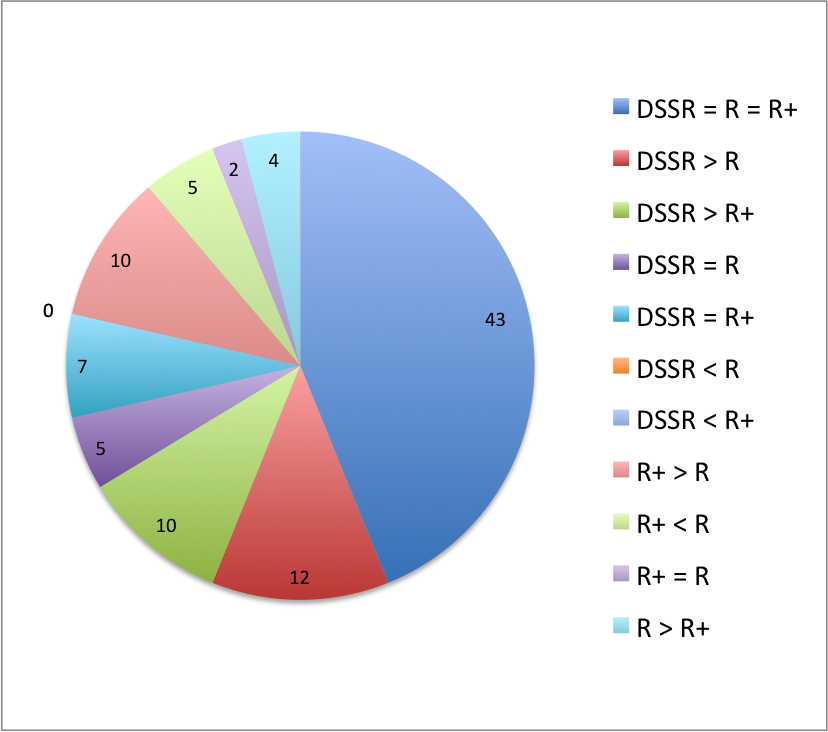
\includegraphics[width=8cm,height=7cm]{pie5.png}
%\caption{Division of result in to categories}
%\label{fig:pie}
%\end{figure}






The first category contain 12 classes where DSSR performed better than R. 
The second category contain 10 classes where DSSR performed better than R+. 
The third category contain 5 classes where DSSR and R performed equally well.
The fourth category contain 7 classes where DSSR and R+ performed equally well. 

The fifth category contain 10 classes where R+ performed better than R.
The sixth category contain 5 classes where R performed better than R+.
The seventh category contain 2 classes where R and R+ performed equally well.
The eighth category contain 4 classes where R performed better than R+.

Category 9 and 10 are interesting because it shows that neither R or nor R+ performed better than DSSR.

The last category is the largest where each strategy performed equally well and found the same number of unique failures after $10^5$ tests. It contain 43 classes.


The answer to this research question is that most classes (72\%) did not exhibit significantly different behaviours independent of the strategy. In 28\% of the cases, the DSSR performed better than R and R+ because DSSR found the highest number of faults and in not a single case R and R+ performed better than DSSR. The result is not unusual because DSSR possess the qualities of both R and R+ strategy with addition of spot sweeping strategy. 


\subsection{Can we pick the best default strategy between R, R+ and DSSR?}
In most cases, results are not different from one strategy to another, but from the analysis of the experimental data we can assess that DSSR has an edge because of spot sweeping feature over R and R+. 

In the next section we also discuss other factors that influence the outcome of such a question such as time taken by each strategy, effect of test duration, number of tests, number of faults and the effect of finding first fault by random strategy on DSSR performance.



%%%%%%%%%%%%%%%%%    DISCUSSION   %%%%%%%%%%%%%%%%%%%%

\section{Discussion}\label{sec:discussion}
\textbf{Time taken by DSSR strategy, Random strategy and Random plus strategy to execute tests:}
To execute an equal number of test cases, DSSR takes slightly more time (up to maximum 5\% overhead) than both pure random and random plus. This is due to maintaining sets of interesting values. The overhead is dependent on our implementation and could also be reduced if needed. 

\textbf{Effect of test duration and number of tests on the results:}
All three techniques have the same potential for finding bugs. If testing infinitely, all techniques should find the same number of unique failures.
So the results will converge the longer (resp. the more tests) testing sessions contain. We suspect however that some of the unique failures found would be extremely long to find using random or random+ only. Further experiments should confirm this point.


\textbf{Effect of number of faults on results:} 
We found that the DSSR strategy performs better when the number of faults is higher in the code. The reason seems to be that when there are more faults, their domains are more connected and DSSR then works better. Further studies might use historical data to pick the best strategy.

\textbf{DSSR strategy dependence on finding the first unique failures early enough:}
During the experiments we found that if the unique failures is not found  quickly enough there is no value added to the list of interesting values and then the test is equivalent random testing. This means that better ways of populating failure-inducing values are needed to leverage DSSR better. As an example, the following piece of code would be unlikely to fail under the current setting:

\begin{lstlisting}
public void test(float value){
 if(value == 34.4445) { 
  10/0; 
 }
}
\end{lstlisting}

In this case, we could add constant literals from the SUT to the list of interesting values in a dynamic fashion. These literals can be obtained from the constant pool in the class files of the SUT.

In the example above the value 34.4445 and its surrounding values would  be added to the list of interesting values before the test starts and the DSSR strategy would find the unique failure right away.

\textbf{DSSR strategy and coverage:} Random strategies typically achieve high level of coverage~\cite{Oriol2010}. It might also be interesting to compare R, R+ and DSSR with respect to the achieved coverage or even to use a DSSR variant that adds a new interesting value and its neighbours when a new branch is reached.


\textbf{Threats to validity:} As usual with such empirical studies, the present work might suffer from a non-representative selection of classes.
The present selection was however made through random selection and objective criteria and it seems unlikely that they would not be representative.

The parameters of the study might also have prompted incorrect results. This is however unlikely due to previous results on random testing~\cite{Oriol2012}.



%%%%%%%%%%%%%%%%%    RW   %%%%%%%%%%%%%%%%%%%%

\section{Related Work}\label{sec:rw}

Random testing is a popular technique with simple algorithm but proven to find subtle faults in complex programs and Java libraries~\cite{Pacheco2005, Csallner2004, Claessen2000a}. Its simplicity, ease of implementation and efficiency in generating test cases make it a best choice for test automation~\cite{Hamlet1994}. Few of the well known automated tools based on random strategy includes Jartege~\cite{Oriat2004}, Eclat~\cite{Pacheco2005}, JCrasher~\cite{Csallner2004}, AutoTest \cite{Ciupa2007, Ciupa2008a} and YETI~\cite{Oriol2010, Oriol2012}  which was used to conduct this research study.

In pursuit of better results and lower overhead, many variations of random strategy have been proposed~\cite{Chen2010, Chen2005, Chan2002, Chen2004a, Chen2003}. Adaptive random testing (ART), Quasi-random testing (QRT) and Restricted Random testing (RRT) achieved better results by selecting test inputs random but evenly spread across the input domain. Similarly Mirror ART and ART through dynamic partitioning increased the performances by reducing the overhead of ART. One of the main reason behind the better performance of these strategies is that even spread of test input increases the chance of exploring the fault patterns present in the input domain.

A more recent research study \cite{Yoo2012} also stress on the effectiveness of data regeneration in close vicinity of the existing test data. Experiments performed showed up to two orders of magnitude more efficient test data generation than the existing techniques. Two major limitation of this study is the availability of pre-existing test cases to regenerate new ones, and increased overhead as it utilise ``meta heuristics search'' based on hill climbing algorithm to regenerate new data. In DSSR no pre-existing test cases are required because it utilises the border values from R+ and regenerate the data very cheap (if x is fault then x + 1, x + 2, x - 1 and x -2 are added) in a dynamic fashion different for each class under test with minimal overhead. 
  
The random+ (R+) strategy~\cite{Leitner2007} is a variation of the random strategy in which interesting values, beside pure random values, are added to the list of test inputs. These interesting values includes border values~\cite{Beizer1990} which have high tendency of finding faults in the given SUT. Results conducted with R+ strategy show significant improvement of pure random strategy. DSSR strategy also rely on R+ strategy in the start until any fault is found where it switches to spot sweeping strategy.

%It is interesting that numerous efforts have been made to discover the fault patterns~\cite{Chen2010, Chen2005, Chan2002, Chen2004a, Chen2003}, etc. but in our knowledge, none has been published on covering/sweeping all the faults lying in a specific pattern once it has been discovered.




A common practice to evaluate performance of newly created or existing strategies is to compare the results obtained (theoretically and empirically) after applying them to similar programs~\cite{Gutjahr1999, Duran1984, Hamlet1990}. Arcuri et al., stress on the use of random testing as a comparison baseline to assess other test strategies \cite{Arcuri2012}. We followed similar procedure and evaluated DSSR against R and R+ under constant conditions.

Qualitas Corpus~\cite{Tempero2010} is a collection of open source java programs maintained for independent empirical research~\cite{Oriol2012, Tempero2010a, Tempero2008}. These projects are carefully selected that spans across the whole set of java applications.


%%%%%%%%%%%%%%%%%    CONCLUSIONS   %%%%%%%%%%%%%%%%%%%%


\section{Conclusions}\label{sec:conc}
The main goal of the present study was to develop a new random strategy which could find more faults in lower number of test cases that would leverage on the assumption that in a significant number of classes, failure domains are contiguous or are very close by. The result is the dirt spot sweeping strategy, a strategy which adds neighbouring values of failure values to a set of preferred values. 

We implemented DSSR as a strategy for the random testing tool YETI and tested thirty times each one of 60 classes from the Qualitas Corpus with each of the three strategies DSSR, R, and R+.We found that for 72\% of the classes all three strategies find the same unique failures, for remaining 28\% DSSR perform better (up to as much as 33\%) then random strategy and (up to as much as 17\%) then random+ strategy.
Overall, DSSR also found 27 more unique failures than random and 11 more unique failures than random+ strategy.

Overall DSSR is a strategy that uncovers more unique failures than both random and random+ strategies. It however achieves this with up to 5\% overhead which is its only downside. It however yields encouraging results and advocates to develop the technique further for settings in which it is significantly better than both R and R+.

%%%%%%%%%%%%%%%%%    ACKNOWDLEGEMENT   %%%%%%%%%%%%%%%%%%%%
\section{Acknowledgments}
The authors thank the Department of Computer Science, University of York for its financial support through the Departmental Overseas Research Scholarship (DORS) award. Authors also thanks Richard Page, for his valuable help and generous support.




%
% The following two commands are all you need in the
% initial runs of your .tex file to
% produce the bibliography for the citations in your paper.
\bibliographystyle{abbrv}
\bibliography{sigproc}  % sigproc.bib is the name of the Bibliography in this case
% You must have a proper ".bib" file
%  and remember to run:
% latex bibtex latex latex
% to resolve all references
%
% ACM needs 'a single self-contained file'!
%
%APPENDICES are optional
%\balancecolumns
\end{document}
